\documentclass[12pt,a4paper]{article}
\usepackage[utf8]{vietnam}
\usepackage{amsmath,amssymb}
\usepackage{tabularx}
\usepackage{tikz}
\usepackage{xcolor}
\usepackage[top=0.6cm, bottom=0.6cm, left=0.6cm, right=0.6cm]{geometry}
\usepackage[dethi]{ex_test}

\SAOPTN{widthSA=2.8,heightSA=0.62}
\setlength{\parskip}{0pt}

% Dong ke cham mo chuan viet tay
\newcommand{\dongke}[1]{%
  \begingroup%
  \setlength{\parskip}{0pt}%
  \baselineskip=18.5pt%
  \vspace{1.0mm}%
  \foreach \i in {1,...,#1}{%
    \noindent{\color{gray!60}\dotfill}\par%
  }%
  \vspace{0.6mm}%
  \endgroup%
}

% Khu vuc bai lam chia 2 cot co vach ngan mo o giua
\newcommand{\dongkeHaiCot}[1]{%
  \par\vspace{0.5mm}%
  \noindent%
  \begin{minipage}[t]{0.485\linewidth}%
    \dongke{#1}%
  \end{minipage}%
  \hfill%
  {\color{gray!60}\vrule}%
  \hfill%
  \begin{minipage}[t]{0.485\linewidth}%
    \dongke{#1}%
  \end{minipage}%
}

% Dinh nghia o bai tap tu luan trong bang
\newcommand{\oBaiTap}[3][5]{%
  \vspace{1.0mm}%
  \noindent\textbf{#2} #3\par%
  \dongke{#1}%
}

\begin{document}
\pagestyle{empty}
% =============================================================================
% ========================= TOAN 8 TUAN 11 BUOI 02 - MA DE 101 =================
% ========================= TRANG 1/2 ==========================================
% =============================================================================
\noindent
\begin{tabularx}{\linewidth}{|X|c|}
\hline
\textbf{PHIẾU KIỂM TRA ĐỊNH KỲ TOÁN 8 - TUẦN 11 - BUỔI 02} & \textbf{Mã đề: 101 - Trang 1/2} \\
\hline
\end{tabularx}

\vspace{1.0mm}

\noindent
\begin{tabularx}{\linewidth}{|p{3.2cm}|X|}
\hline
\centering\textbf{ĐIỂM SỐ} & \centering\textbf{LỜI NHẬN XÉT CỦA THẦY CÔ} \tabularnewline
\hline
\rule{0pt}{1.8cm} & \tabularnewline
\hline
\end{tabularx}

\vspace{1.2mm}
\noindent\textbf{Câu 1 (0,25 điểm).} Cho hai đoạn thẳng $AB = 6\text{ cm}, CD = 8\text{ cm}$. Tỉ số $\dfrac{AB}{CD} =$ \shortans{\dfrac{3}{4}}\par\vspace{3.0mm}
\noindent\textbf{Câu 2 (0,25 điểm).} Cho $\Delta ABC$ có $DE \parallel BC$, $AD = 3\text{ cm}, DB = 2\text{ cm}, AE = 6\text{ cm}$. Khi đó $EC =$ \shortans{4\text{ cm}}\par\vspace{3.0mm}
\noindent\textbf{Câu 3 (0,25 điểm).} Cho $\Delta ABC$ có $MN \parallel BC$, $\dfrac{AM}{AB} = \dfrac{2}{3}, BC = 15\text{ cm}$. Khi đó $MN =$ \shortans{10\text{ cm}}\par\vspace{3.0mm}
\noindent\textbf{Câu 4 (0,25 điểm).} Kết quả của phép nhân $2x(3x^2 - 4x + 1)$ là: \shortans{6x^3 - 8x^2 + 2x}\par\vspace{3.0mm}
\noindent\textbf{Câu 5 (0,25 điểm).} Khai triển hằng đẳng thức $(2x - 3)^2$, ta được kết quả là: \shortans{4x^2 - 12x + 9}\par\vspace{3.0mm}
\noindent\textbf{Câu 6 (0,25 điểm).} Phân tích đa thức $5x^2 - 10xy$ thành nhân tử, ta được: \shortans{5x(x - 2y)}\par\vspace{3.0mm}
\noindent\textbf{Câu 7 (0,25 điểm).} Phân tích đa thức $9x^2 - 25$ thành nhân tử, ta được: \shortans{(3x - 5)(3x + 5)}\par\vspace{3.0mm}
\noindent\textbf{Câu 8 (0,25 điểm).} Tính nhanh giá trị biểu thức $73^2 + 27^2 + 54 \cdot 73 =$ \shortans{10\,000}\par\vspace{3.0mm}
\noindent\textbf{Câu 9 (0,25 điểm).} Cọc cao $2\text{ m}$ bóng $1{,}5\text{ m}$. Cây có bóng $6\text{ m}$. Chiều cao cây là: \shortans{8\text{ m}}\par\vspace{3.0mm}
\noindent\textbf{Câu 10 (0,25 điểm).} Cho $\Delta ABC$, $M \in AB, N \in AC$. ĐK để $MN \parallel BC$ là: \shortans{\dfrac{AM}{MB} = \dfrac{AN}{NC}}\par\vspace{3.0mm}
\vspace{0.4mm}
\noindent\textbf{Câu 11 (3,0 điểm). Thực hiện các phép tính sau:}
\vspace{0.6mm}

\noindent
\begin{tabularx}{\linewidth}{|X|X|}
\hline
\oBaiTap[5]{a) (0,5 điểm)}{$(3x^2y - 2xy^2) + (2x^2y + 5xy^2)$} & 
\oBaiTap[5]{b) (0,5 điểm)}{$(5x^3 - 3x^2 + 4) - (2x^3 - 3x^2 - 5)$} \\
\hline
\oBaiTap[5]{c) (0,5 điểm)}{$2x^2(3x^2 - 4x + 1)$} & 
\oBaiTap[5]{d) (0,5 điểm)}{$(2x - 3)(x^2 - 2x + 1)$} \\
\hline
\oBaiTap[5]{e) (0,5 điểm)}{$(12x^4y^3 - 8x^3y^2) : 4x^2y^2$} & 
\oBaiTap[5]{f) (0,5 điểm)}{$(2x^3 - 5x^2 + 6x - 2) : (2x - 1)$} \\
\hline
\end{tabularx}

\newpage
% =============================================================================
% ========================= TOAN 8 TUAN 11 BUOI 02 - MA DE 101 =================
% ========================= TRANG 2/2 ==========================================
% =============================================================================
\noindent
\begin{tabularx}{\linewidth}{|X|c|}
\hline
\textbf{TOÁN 8 - TUẦN 11 - BUỔI 02} & \textbf{Mã đề: 101 - Trang 2/2} \\
\hline
\end{tabularx}

\vspace{1.2mm}

\noindent\textbf{Câu 12 (2,0 điểm). Phân tích các đa thức sau thành nhân tử:}
\vspace{0.6mm}

\noindent
\begin{tabularx}{\linewidth}{|X|X|}
\hline
\oBaiTap[5]{a) (0,5 điểm)}{$4x^2 - 12x$} & 
\oBaiTap[5]{b) (0,5 điểm)}{$9x^2 - 16$} \\
\hline
\oBaiTap[5]{c) (0,5 điểm)}{$xy - 2y + 3x - 6$} & 
\oBaiTap[5]{d) (0,5 điểm)}{$x^2 - 2xy + y^2 - 25$} \\
\hline
\end{tabularx}

\vspace{1.2mm}

\noindent
\begin{tabularx}{\linewidth}{|X|}
\hline
\vspace{0.5mm}
\begin{minipage}[t]{0.57\linewidth}
\vspace{0pt}
\textbf{Câu 13 (2,0 điểm).} Cho tam giác $ABC$ nhọn ($AB < AC$), có $AB = 12\text{ cm}, AC = 15\text{ cm}$. Trên cạnh $AB$ lấy điểm $D$ sao cho $AD = 4\text{ cm}$, trên cạnh $AC$ lấy điểm $E$ sao cho $AE = 5\text{ cm}$.\par\vspace{0.4mm}
\textbf{a)} (1,0 điểm) Chứng minh rằng $DE \parallel BC$.\par\vspace{0.4mm}
\textbf{b)} (1,0 điểm) Biết $BC = 18\text{ cm}$. Tính độ dài đoạn thẳng $DE$ và độ dài đoạn thẳng $DB$.
\end{minipage}\hfill
\begin{minipage}[t]{0.41\linewidth}
\vspace{0pt}\centering
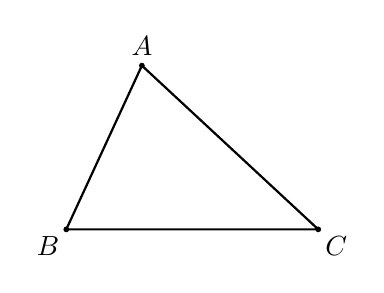
\begin{tikzpicture}[scale=0.8, >=stealth, line join=round, line cap=round]
  \coordinate (B) at (0, 0);
  \coordinate (C) at (4.0, 0);
  \coordinate (A) at (1.2, 2.6);

  \draw[thick] (A) -- (B) -- (C) -- cycle;

  \fill (A) circle (1.3pt) node[above] {$A$};
  \fill (B) circle (1.3pt) node[below left=-1pt] {$B$};
  \fill (C) circle (1.3pt) node[below right=-1pt] {$C$};
\end{tikzpicture}
\end{minipage}\par
\vspace{0.4mm}
\noindent\textit{Bài giải:}\dongkeHaiCot{10}
\\ \hline
\end{tabularx}

\vspace{1.2mm}

\noindent
\begin{tabularx}{\linewidth}{|X|}
\hline
\vspace{0.5mm}
\textbf{Câu 14 (0,5 điểm).} Tìm giá trị nhỏ nhất của biểu thức: $A = x^2 - 6x + 13$.\par
\vspace{0.4mm}
\noindent\textit{Bài giải:}\dongkeHaiCot{7}
\\ \hline
\end{tabularx}

\newpage
% =============================================================================
% ========================= TOAN 8 TUAN 11 BUOI 02 - MA DE 102 =================
% ========================= TRANG 1/2 ==========================================
% =============================================================================
\noindent
\begin{tabularx}{\linewidth}{|X|c|}
\hline
\textbf{PHIẾU KIỂM TRA ĐỊNH KỲ TOÁN 8 - TUẦN 11 - BUỔI 02} & \textbf{Mã đề: 102 - Trang 1/2} \\
\hline
\end{tabularx}

\vspace{1.0mm}

\noindent
\begin{tabularx}{\linewidth}{|p{3.2cm}|X|}
\hline
\centering\textbf{ĐIỂM SỐ} & \centering\textbf{LỜI NHẬN XÉT CỦA THẦY CÔ} \tabularnewline
\hline
\rule{0pt}{1.8cm} & \tabularnewline
\hline
\end{tabularx}

\vspace{1.2mm}
\noindent\textbf{Câu 1 (0,25 điểm).} Cho hai đoạn thẳng $MN = 4\text{ cm}, PQ = 10\text{ cm}$. Tỉ số $\dfrac{MN}{PQ} =$ \shortans{\dfrac{2}{5}}\par\vspace{3.0mm}
\noindent\textbf{Câu 2 (0,25 điểm).} Cho $\Delta ABC$ có $DE \parallel BC$, $AD = 2\text{ cm}, DB = 4\text{ cm}, AE = 3\text{ cm}$. Khi đó $EC =$ \shortans{6\text{ cm}}\par\vspace{3.0mm}
\noindent\textbf{Câu 3 (0,25 điểm).} Cho $\Delta ABC$ có $MN \parallel BC$, $\dfrac{AM}{AB} = \dfrac{3}{4}, BC = 16\text{ cm}$. Khi đó $MN =$ \shortans{12\text{ cm}}\par\vspace{3.0mm}
\noindent\textbf{Câu 4 (0,25 điểm).} Kết quả của phép nhân $3x(2x^2 - 5x + 2)$ là: \shortans{6x^3 - 15x^2 + 6x}\par\vspace{3.0mm}
\noindent\textbf{Câu 5 (0,25 điểm).} Khai triển hằng đẳng thức $(3x - 2)^2$, ta được kết quả là: \shortans{9x^2 - 12x + 4}\par\vspace{3.0mm}
\noindent\textbf{Câu 6 (0,25 điểm).} Phân tích đa thức $6x^2 - 12xy$ thành nhân tử, ta được: \shortans{6x(x - 2y)}\par\vspace{3.0mm}
\noindent\textbf{Câu 7 (0,25 điểm).} Phân tích đa thức $4x^2 - 49$ thành nhân tử, ta được: \shortans{(2x - 7)(2x + 7)}\par\vspace{3.0mm}
\noindent\textbf{Câu 8 (0,25 điểm).} Tính nhanh giá trị biểu thức $84^2 + 16^2 + 32 \cdot 84 =$ \shortans{10\,000}\par\vspace{3.0mm}
\noindent\textbf{Câu 9 (0,25 điểm).} Cọc cao $2\text{ m}$ bóng $1{,}2\text{ m}$. Tháp có bóng $9\text{ m}$. Chiều cao tháp là: \shortans{15\text{ m}}\par\vspace{3.0mm}
\noindent\textbf{Câu 10 (0,25 điểm).} Cho $\Delta ABC$, $D \in AB, E \in AC$. ĐK để $DE \parallel BC$ là: \shortans{\dfrac{AD}{AB} = \dfrac{AE}{AC}}\par\vspace{3.0mm}
\vspace{0.4mm}
\noindent\textbf{Câu 11 (3,0 điểm). Thực hiện các phép tính sau:}
\vspace{0.6mm}

\noindent
\begin{tabularx}{\linewidth}{|X|X|}
\hline
\oBaiTap[5]{a) (0,5 điểm)}{$(4x^2y - 3xy^2) + (x^2y + 6xy^2)$} & 
\oBaiTap[5]{b) (0,5 điểm)}{$(6x^3 - 4x^2 + 5) - (2x^3 - 4x^2 - 3)$} \\
\hline
\oBaiTap[5]{c) (0,5 điểm)}{$3x^2(2x^2 - 3x + 1)$} & 
\oBaiTap[5]{d) (0,5 điểm)}{$(2x - 1)(x^2 - 3x + 2)$} \\
\hline
\oBaiTap[5]{e) (0,5 điểm)}{$(15x^4y^3 - 9x^3y^2) : 3x^2y^2$} & 
\oBaiTap[5]{f) (0,5 điểm)}{$(2x^3 - 7x^2 + 7x - 2) : (2x - 1)$} \\
\hline
\end{tabularx}

\newpage
% =============================================================================
% ========================= TOAN 8 TUAN 11 BUOI 02 - MA DE 102 =================
% ========================= TRANG 2/2 ==========================================
% =============================================================================
\noindent
\begin{tabularx}{\linewidth}{|X|c|}
\hline
\textbf{TOÁN 8 - TUẦN 11 - BUỔI 02} & \textbf{Mã đề: 102 - Trang 2/2} \\
\hline
\end{tabularx}

\vspace{1.2mm}

\noindent\textbf{Câu 12 (2,0 điểm). Phân tích các đa thức sau thành nhân tử:}
\vspace{0.6mm}

\noindent
\begin{tabularx}{\linewidth}{|X|X|}
\hline
\oBaiTap[5]{a) (0,5 điểm)}{$5x^2 - 15x$} & 
\oBaiTap[5]{b) (0,5 điểm)}{$16x^2 - 25$} \\
\hline
\oBaiTap[5]{c) (0,5 điểm)}{$xy - 3y + 4x - 12$} & 
\oBaiTap[5]{d) (0,5 điểm)}{$x^2 - 2xy + y^2 - 36$} \\
\hline
\end{tabularx}

\vspace{1.2mm}

\noindent
\begin{tabularx}{\linewidth}{|X|}
\hline
\vspace{0.5mm}
\begin{minipage}[t]{0.57\linewidth}
\vspace{0pt}
\textbf{Câu 13 (2,0 điểm).} Cho tam giác $MNP$ nhọn ($MN < MP$), có $MN = 12\text{ cm}, MP = 16\text{ cm}$. Trên cạnh $MN$ lấy điểm $D$ sao cho $MD = 3\text{ cm}$, trên cạnh $MP$ lấy điểm $E$ sao cho $ME = 4\text{ cm}$.\par\vspace{0.4mm}
\textbf{a)} (1,0 điểm) Chứng minh rằng $DE \parallel NP$.\par\vspace{0.4mm}
\textbf{b)} (1,0 điểm) Biết $NP = 20\text{ cm}$. Tính độ dài đoạn thẳng $DE$ và độ dài đoạn thẳng $DN$.
\end{minipage}\hfill
\begin{minipage}[t]{0.41\linewidth}
\vspace{0pt}\centering
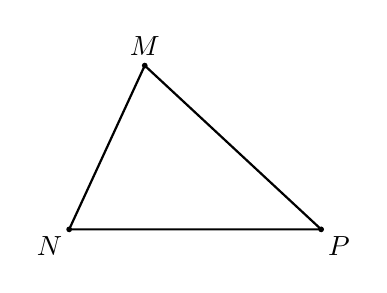
\begin{tikzpicture}[scale=0.8, >=stealth, line join=round, line cap=round]
  \coordinate (N) at (0, 0);
  \coordinate (P) at (4.0, 0);
  \coordinate (M) at (1.2, 2.6);

  \draw[thick] (M) -- (N) -- (P) -- cycle;

  \fill (M) circle (1.3pt) node[above] {$M$};
  \fill (N) circle (1.3pt) node[below left=-1pt] {$N$};
  \fill (P) circle (1.3pt) node[below right=-1pt] {$P$};
\end{tikzpicture}
\end{minipage}\par
\vspace{0.4mm}
\noindent\textit{Bài giải:}\dongkeHaiCot{10}
\\ \hline
\end{tabularx}

\vspace{1.2mm}

\noindent
\begin{tabularx}{\linewidth}{|X|}
\hline
\vspace{0.5mm}
\textbf{Câu 14 (0,5 điểm).} Tìm giá trị nhỏ nhất của biểu thức: $A = x^2 - 8x + 25$.\par
\vspace{0.4mm}
\noindent\textit{Bài giải:}\dongkeHaiCot{7}
\\ \hline
\end{tabularx}

\newpage
% =============================================================================
% ========================= TOAN 8 TUAN 11 BUOI 02 - MA DE 103 =================
% ========================= TRANG 1/2 ==========================================
% =============================================================================
\noindent
\begin{tabularx}{\linewidth}{|X|c|}
\hline
\textbf{PHIẾU KIỂM TRA ĐỊNH KỲ TOÁN 8 - TUẦN 11 - BUỔI 02} & \textbf{Mã đề: 103 - Trang 1/2} \\
\hline
\end{tabularx}

\vspace{1.0mm}

\noindent
\begin{tabularx}{\linewidth}{|p{3.2cm}|X|}
\hline
\centering\textbf{ĐIỂM SỐ} & \centering\textbf{LỜI NHẬN XÉT CỦA THẦY CÔ} \tabularnewline
\hline
\rule{0pt}{1.8cm} & \tabularnewline
\hline
\end{tabularx}

\vspace{1.2mm}
\noindent\textbf{Câu 1 (0,25 điểm).} Cho hai đoạn thẳng $AB = 9\text{ cm}, CD = 12\text{ cm}$. Tỉ số $\dfrac{AB}{CD} =$ \shortans{\dfrac{3}{4}}\par\vspace{3.0mm}
\noindent\textbf{Câu 2 (0,25 điểm).} Cho $\Delta ABC$ có $DE \parallel BC$, $AD = 4\text{ cm}, DB = 2\text{ cm}, AE = 8\text{ cm}$. Khi đó $EC =$ \shortans{4\text{ cm}}\par\vspace{3.0mm}
\noindent\textbf{Câu 3 (0,25 điểm).} Cho $\Delta ABC$ có $MN \parallel BC$, $\dfrac{AM}{AB} = \dfrac{2}{5}, BC = 20\text{ cm}$. Khi đó $MN =$ \shortans{8\text{ cm}}\par\vspace{3.0mm}
\noindent\textbf{Câu 4 (0,25 điểm).} Kết quả của phép nhân $2x(4x^2 - 3x + 2)$ là: \shortans{8x^3 - 6x^2 + 4x}\par\vspace{3.0mm}
\noindent\textbf{Câu 5 (0,25 điểm).} Khai triển hằng đẳng thức $(2x - 5)^2$, ta được kết quả là: \shortans{4x^2 - 20x + 25}\par\vspace{3.0mm}
\noindent\textbf{Câu 6 (0,25 điểm).} Phân tích đa thức $4x^2 - 12xy$ thành nhân tử, ta được: \shortans{4x(x - 3y)}\par\vspace{3.0mm}
\noindent\textbf{Câu 7 (0,25 điểm).} Phân tích đa thức $16x^2 - 9$ thành nhân tử, ta được: \shortans{(4x - 3)(4x + 3)}\par\vspace{3.0mm}
\noindent\textbf{Câu 8 (0,25 điểm).} Tính nhanh giá trị biểu thức $68^2 + 32^2 + 64 \cdot 68 =$ \shortans{10\,000}\par\vspace{3.0mm}
\noindent\textbf{Câu 9 (0,25 điểm).} Cọc cao $1{,}8\text{ m}$ bóng $1{,}2\text{ m}$. Cây có bóng $8\text{ m}$. Chiều cao cây là: \shortans{12\text{ m}}\par\vspace{3.0mm}
\noindent\textbf{Câu 10 (0,25 điểm).} Cho $\Delta ABC$, $M \in AB, N \in AC$. ĐK để $MN \parallel BC$ là: \shortans{\dfrac{AM}{AB} = \dfrac{AN}{AC}}\par\vspace{3.0mm}
\vspace{0.4mm}
\noindent\textbf{Câu 11 (3,0 điểm). Thực hiện các phép tính sau:}
\vspace{0.6mm}

\noindent
\begin{tabularx}{\linewidth}{|X|X|}
\hline
\oBaiTap[5]{a) (0,5 điểm)}{$(5x^2y - 4xy^2) + (2x^2y + 7xy^2)$} & 
\oBaiTap[5]{b) (0,5 điểm)}{$(7x^3 - 5x^2 + 6) - (3x^3 - 5x^2 - 4)$} \\
\hline
\oBaiTap[5]{c) (0,5 điểm)}{$2x^2(4x^2 - 3x + 2)$} & 
\oBaiTap[5]{d) (0,5 điểm)}{$(3x - 1)(x^2 - 2x + 1)$} \\
\hline
\oBaiTap[5]{e) (0,5 điểm)}{$(16x^4y^3 - 12x^3y^2) : 4x^2y^2$} & 
\oBaiTap[5]{f) (0,5 điểm)}{$(3x^3 - 7x^2 + 5x - 1) : (3x - 1)$} \\
\hline
\end{tabularx}

\newpage
% =============================================================================
% ========================= TOAN 8 TUAN 11 BUOI 02 - MA DE 103 =================
% ========================= TRANG 2/2 ==========================================
% =============================================================================
\noindent
\begin{tabularx}{\linewidth}{|X|c|}
\hline
\textbf{TOÁN 8 - TUẦN 11 - BUỔI 02} & \textbf{Mã đề: 103 - Trang 2/2} \\
\hline
\end{tabularx}

\vspace{1.2mm}

\noindent\textbf{Câu 12 (2,0 điểm). Phân tích các đa thức sau thành nhân tử:}
\vspace{0.6mm}

\noindent
\begin{tabularx}{\linewidth}{|X|X|}
\hline
\oBaiTap[5]{a) (0,5 điểm)}{$6x^2 - 18x$} & 
\oBaiTap[5]{b) (0,5 điểm)}{$25x^2 - 4$} \\
\hline
\oBaiTap[5]{c) (0,5 điểm)}{$xy - 4y + 2x - 8$} & 
\oBaiTap[5]{d) (0,5 điểm)}{$x^2 - 2xy + y^2 - 49$} \\
\hline
\end{tabularx}

\vspace{1.2mm}

\noindent
\begin{tabularx}{\linewidth}{|X|}
\hline
\vspace{0.5mm}
\begin{minipage}[t]{0.57\linewidth}
\vspace{0pt}
\textbf{Câu 13 (2,0 điểm).} Cho tam giác $ABC$ nhọn ($AB < AC$), có $AB = 10\text{ cm}, AC = 15\text{ cm}$. Trên cạnh $AB$ lấy điểm $M$ sao cho $AM = 4\text{ cm}$, trên cạnh $AC$ lấy điểm $N$ sao cho $AN = 6\text{ cm}$.\par\vspace{0.4mm}
\textbf{a)} (1,0 điểm) Chứng minh rằng $MN \parallel BC$.\par\vspace{0.4mm}
\textbf{b)} (1,0 điểm) Biết $BC = 25\text{ cm}$. Tính độ dài đoạn thẳng $MN$ và độ dài đoạn thẳng $MB$.
\end{minipage}\hfill
\begin{minipage}[t]{0.41\linewidth}
\vspace{0pt}\centering
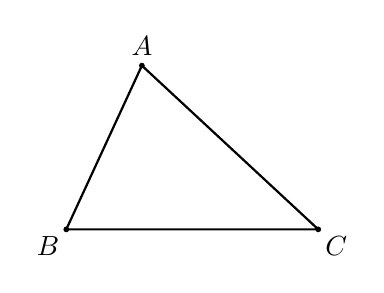
\begin{tikzpicture}[scale=0.8, >=stealth, line join=round, line cap=round]
  \coordinate (B) at (0, 0);
  \coordinate (C) at (4.0, 0);
  \coordinate (A) at (1.2, 2.6);

  \draw[thick] (A) -- (B) -- (C) -- cycle;

  \fill (A) circle (1.3pt) node[above] {$A$};
  \fill (B) circle (1.3pt) node[below left=-1pt] {$B$};
  \fill (C) circle (1.3pt) node[below right=-1pt] {$C$};
\end{tikzpicture}
\end{minipage}\par
\vspace{0.4mm}
\noindent\textit{Bài giải:}\dongkeHaiCot{10}
\\ \hline
\end{tabularx}

\vspace{1.2mm}

\noindent
\begin{tabularx}{\linewidth}{|X|}
\hline
\vspace{0.5mm}
\textbf{Câu 14 (0,5 điểm).} Tìm giá trị nhỏ nhất của biểu thức: $A = x^2 - 10x + 31$.\par
\vspace{0.4mm}
\noindent\textit{Bài giải:}\dongkeHaiCot{7}
\\ \hline
\end{tabularx}

\newpage
% =============================================================================
% ========================= TOAN 8 TUAN 11 BUOI 02 - MA DE 104 =================
% ========================= TRANG 1/2 ==========================================
% =============================================================================
\noindent
\begin{tabularx}{\linewidth}{|X|c|}
\hline
\textbf{PHIẾU KIỂM TRA ĐỊNH KỲ TOÁN 8 - TUẦN 11 - BUỔI 02} & \textbf{Mã đề: 104 - Trang 1/2} \\
\hline
\end{tabularx}

\vspace{1.0mm}

\noindent
\begin{tabularx}{\linewidth}{|p{3.2cm}|X|}
\hline
\centering\textbf{ĐIỂM SỐ} & \centering\textbf{LỜI NHẬN XÉT CỦA THẦY CÔ} \tabularnewline
\hline
\rule{0pt}{1.8cm} & \tabularnewline
\hline
\end{tabularx}

\vspace{1.2mm}
\noindent\textbf{Câu 1 (0,25 điểm).} Cho hai đoạn thẳng $EF = 6\text{ cm}, GH = 15\text{ cm}$. Tỉ số $\dfrac{EF}{GH} =$ \shortans{\dfrac{2}{5}}\par\vspace{3.0mm}
\noindent\textbf{Câu 2 (0,25 điểm).} Cho $\Delta ABC$ có $DE \parallel BC$, $AD = 3\text{ cm}, DB = 6\text{ cm}, AE = 4\text{ cm}$. Khi đó $EC =$ \shortans{8\text{ cm}}\par\vspace{3.0mm}
\noindent\textbf{Câu 3 (0,25 điểm).} Cho $\Delta ABC$ có $MN \parallel BC$, $\dfrac{AM}{AB} = \dfrac{3}{5}, BC = 25\text{ cm}$. Khi đó $MN =$ \shortans{15\text{ cm}}\par\vspace{3.0mm}
\noindent\textbf{Câu 4 (0,25 điểm).} Kết quả của phép nhân $3x(3x^2 - 4x + 1)$ là: \shortans{9x^3 - 12x^2 + 3x}\par\vspace{3.0mm}
\noindent\textbf{Câu 5 (0,25 điểm).} Khai triển hằng đẳng thức $(3x - 1)^2$, ta được kết quả là: \shortans{9x^2 - 6x + 1}\par\vspace{3.0mm}
\noindent\textbf{Câu 6 (0,25 điểm).} Phân tích đa thức $7x^2 - 14xy$ thành nhân tử, ta được: \shortans{7x(x - 2y)}\par\vspace{3.0mm}
\noindent\textbf{Câu 7 (0,25 điểm).} Phân tích đa thức $25x^2 - 36$ thành nhân tử, ta được: \shortans{(5x - 6)(5x + 6)}\par\vspace{3.0mm}
\noindent\textbf{Câu 8 (0,25 điểm).} Tính nhanh giá trị biểu thức $77^2 + 23^2 + 46 \cdot 77 =$ \shortans{10\,000}\par\vspace{3.0mm}
\noindent\textbf{Câu 9 (0,25 điểm).} Cọc cao $2\text{ m}$ bóng $1{,}5\text{ m}$. Cột cờ có bóng $7{,}5\text{ m}$. Chiều cao cột cờ là: \shortans{10\text{ m}}\par\vspace{3.0mm}
\noindent\textbf{Câu 10 (0,25 điểm).} Cho $\Delta ABC$, $D \in AB, E \in AC$. ĐK để $DE \parallel BC$ là: \shortans{\dfrac{AD}{DB} = \dfrac{AE}{EC}}\par\vspace{3.0mm}
\vspace{0.4mm}
\noindent\textbf{Câu 11 (3,0 điểm). Thực hiện các phép tính sau:}
\vspace{0.6mm}

\noindent
\begin{tabularx}{\linewidth}{|X|X|}
\hline
\oBaiTap[5]{a) (0,5 điểm)}{$(2x^2y - 5xy^2) + (3x^2y + 8xy^2)$} & 
\oBaiTap[5]{b) (0,5 điểm)}{$(5x^3 - 2x^2 + 7) - (x^3 - 2x^2 - 1)$} \\
\hline
\oBaiTap[5]{c) (0,5 điểm)}{$3x^2(3x^2 - 4x + 2)$} & 
\oBaiTap[5]{d) (0,5 điểm)}{$(2x - 3)(x^2 - 3x + 2)$} \\
\hline
\oBaiTap[5]{e) (0,5 điểm)}{$(18x^4y^3 - 12x^3y^2) : 6x^2y^2$} & 
\oBaiTap[5]{f) (0,5 điểm)}{$(2x^3 - 9x^2 + 13x - 6) : (2x - 3)$} \\
\hline
\end{tabularx}

\newpage
% =============================================================================
% ========================= TOAN 8 TUAN 11 BUOI 02 - MA DE 104 =================
% ========================= TRANG 2/2 ==========================================
% =============================================================================
\noindent
\begin{tabularx}{\linewidth}{|X|c|}
\hline
\textbf{TOÁN 8 - TUẦN 11 - BUỔI 02} & \textbf{Mã đề: 104 - Trang 2/2} \\
\hline
\end{tabularx}

\vspace{1.2mm}

\noindent\textbf{Câu 12 (2,0 điểm). Phân tích các đa thức sau thành nhân tử:}
\vspace{0.6mm}

\noindent
\begin{tabularx}{\linewidth}{|X|X|}
\hline
\oBaiTap[5]{a) (0,5 điểm)}{$3x^2 - 12x$} & 
\oBaiTap[5]{b) (0,5 điểm)}{$4x^2 - 49$} \\
\hline
\oBaiTap[5]{c) (0,5 điểm)}{$xy - 5y + 3x - 15$} & 
\oBaiTap[5]{d) (0,5 điểm)}{$x^2 - 2xy + y^2 - 64$} \\
\hline
\end{tabularx}

\vspace{1.2mm}

\noindent
\begin{tabularx}{\linewidth}{|X|}
\hline
\vspace{0.5mm}
\begin{minipage}[t]{0.57\linewidth}
\vspace{0pt}
\textbf{Câu 13 (2,0 điểm).} Cho tam giác $DEF$ nhọn ($DE < DF$), có $DE = 12\text{ cm}, DF = 18\text{ cm}$. Trên cạnh $DE$ lấy điểm $M$ sao cho $DM = 4\text{ cm}$, trên cạnh $DF$ lấy điểm $N$ sao cho $DN = 6\text{ cm}$.\par\vspace{0.4mm}
\textbf{a)} (1,0 điểm) Chứng minh rằng $MN \parallel EF$.\par\vspace{0.4mm}
\textbf{b)} (1,0 điểm) Biết $EF = 21\text{ cm}$. Tính độ dài đoạn thẳng $MN$ và độ dài đoạn thẳng $ME$.
\end{minipage}\hfill
\begin{minipage}[t]{0.41\linewidth}
\vspace{0pt}\centering
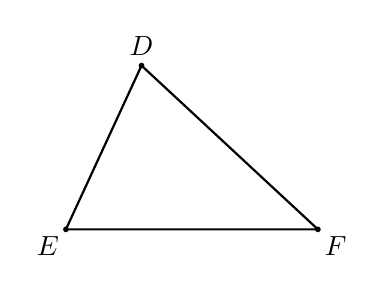
\begin{tikzpicture}[scale=0.8, >=stealth, line join=round, line cap=round]
  \coordinate (E) at (0, 0);
  \coordinate (F) at (4.0, 0);
  \coordinate (D) at (1.2, 2.6);

  \draw[thick] (D) -- (E) -- (F) -- cycle;

  \fill (D) circle (1.3pt) node[above] {$D$};
  \fill (E) circle (1.3pt) node[below left=-1pt] {$E$};
  \fill (F) circle (1.3pt) node[below right=-1pt] {$F$};
\end{tikzpicture}
\end{minipage}\par
\vspace{0.4mm}
\noindent\textit{Bài giải:}\dongkeHaiCot{10}
\\ \hline
\end{tabularx}

\vspace{1.2mm}

\noindent
\begin{tabularx}{\linewidth}{|X|}
\hline
\vspace{0.5mm}
\textbf{Câu 14 (0,5 điểm).} Tìm giá trị nhỏ nhất của biểu thức: $A = x^2 - 4x + 15$.\par
\vspace{0.4mm}
\noindent\textit{Bài giải:}\dongkeHaiCot{7}
\\ \hline
\end{tabularx}
\end{document}
